\section{Durchführung und Aufbau}
\label{sec:Durchführung}

\subsection{Voreinstellung der Schwingkreise}
Die beiden Schwingkreise besitzten nicht dieselbe Resonanzfrequenz, deshalb müssen sie zunächst aufeinander abgestimmt werden. Dazu wird zunächst die Resonanzfrequenz des fest abgestimmten Schwingkreises bestimmt, dies geschieht mit der in Abbildung \ref{fig:ResFrequenz} dargestellten Schaltung.

\begin{figure}[H]
  \centering
  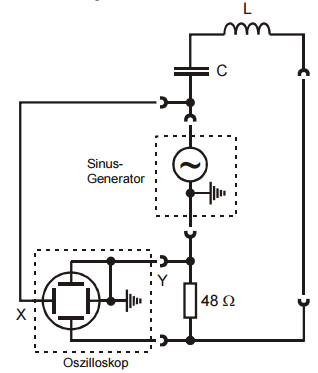
\includegraphics[height=6cm]{picture/BestimmungDerResFrequenz.PNG}
  \caption{Messschaltung zur genauen Bestimmung der Resonanzfrequenz eines Schwingkreises \cite{sample}.}
  \label{fig:ResFrequenz}
\end{figure}

Für eine grobe Abschätzung der Resonanzfrequenz wird die Frequenz gesucht, bei der ein Strom Maximum auftritt. Für eine genauere Bestimmung der Frequenz wird das Oszilloskop in den XY-Betrieb umgeschaltet, es wird die Spannung des Generators auf den X-Eingang gegeben und die Spannung an dem Widerstand auf den Y-Eingang. Die beiden Schwingungen sind in Phase wenn die Lissajous-Figur in eine Gerade übergeht. Diese Frequenz wird notiert und die Schaltung wird nun mit dem abstimmbaren Schwingkreis aufgebaut. Nun wird die in den Schwingkreis eingebaute Kapazität solange verändert bis sich die Lissajous-Figur wieder einer Geraden annähert. Sobald diese Einstellung gefunden wurde, wird diese für alle weiteren Versuche beibehalten.

\subsection{Messprogramm}

\subsubsection{Beobachtung des Energieaustausches}
 Für diesen Aufgabenteil wird die in Abbildung \ref{fig:Blub} dargestellt Schaltung aufgebaut.

 \begin{figure}[H]
   \centering
   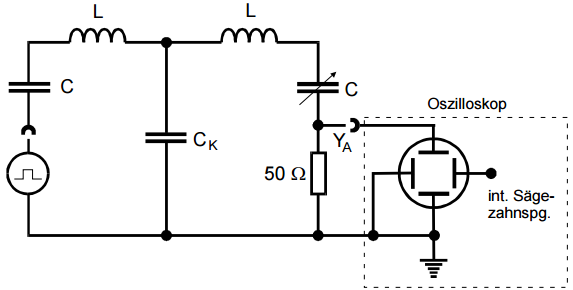
\includegraphics[height=5cm]{picture/Schwebefrequenz.PNG}
   \caption{Schaltung zur Beobachtung des Energieaustausches \cite{sample}.}
   \label{fig:Blub}
 \end{figure}

Nun wird der linke Schwingkreis mit einem Rechteckimpuls angeregt. Die Änderung des Stromes wird über den Spannungsabfall am 48 $\Omega$ Widerstand auf dem Oszilloskop sichtbar gemacht. Auf dem Oszilloskop lassen sich nun Schwebungen, wie in Abbildung \ref{fig:SchFre} dargestellt, erkennen. Nun wird das Verhältniss der Schwebungs- und der Schwingungsfrequenz bestimmt. Dafür werden die Maxima der Schwingungsfrequenz in einer Schwebung gezählt. Dies wird für unterschiedliche Koppelkondesatoren wiederholt, um ein Zusammenhang zwischen dem Frequenzverhältniss und der Kapazität des Kondensatoren zu erkennen.

\subsubsection{Bestimmung der Fundamentalfrequenzen über Lissajous-Figuren}
Es wird die Schaltung aus dem vorherigen Versuch übernommen, allerdings wird nun eine Sinusschwingung verwendet. Außerdem wird die Generatorspannung an den X-Eingang des Oszilloskops gegeben und das Oszilloskop wird auf den XY-Betrieb gestellt, dadurch sind nun wieder Lissajous-Figuren zu erkennen. Die Frequenzen, bei denen die Lissajous-Figuren in eine Gerade übergehen, sind die Fundamentalfrequenzen.\\
Dies wird wieder für unterschiedliche Kapazitäten des Koppelkondensators wiederholt.

\subsubsection{Bestimmung der Fundamentalfrequenzen über die Sweep-Methode}
Bei diesem Versuch wird die Schaltung aus Abbildung \ref{fig:Blub} übernommen. Allerdings wird dieses mal keine konstante Sinusschwingung verwendet, sondern eine in der Frequenz ansteigende Sinusschwingung, ein sogenannter Sweep. Bedeutet, dass die Sinusschingung bei einer Startfrequenz anfängt und über einen Zeitraum linear bis zur Endfrequenz ansteigt. Die Start- und Endfrequenzen werden so gewählt, dass die Fundamentalfrequenzen innerhalb dieses Bereiches liegen. Das Oszilloskop wird so angeschlossen das es die Spannung an dem 48 $\Omega$ Widerstand abnimmt. Desweiteren soll das Bild nach genau einem Sweep einfrieren, damit die Zeitabstände zwischen dem Start des Sweaps und den beiden Maxima gemessen werden können. Dies geschieht mit Hilfe der Cursor-Funktion des Oszilloskops. Die Beiden Maxima stellen in diesem Fall die Fundamentalfrequenzen bzw. Resonanzfrequenzen da. Aus den Zeitabständen können nun die Fundamentalfrequenzen berechnet werden.
